\documentclass[final]{beamer}
\usepackage[T1]{fontenc}
\usepackage{lmodern}
\usepackage[size=custom,width=121,height=91,scale=1.0]{beamerposter}
\usetheme{gemini}
\usecolortheme{ox}
\usepackage{graphicx}
\usepackage{booktabs}
\usepackage{tikz}
\usepackage{pgfplots}
\pgfplotsset{compat=1.14}
\usepackage{anyfontsize}
\usepackage{minted}

\usepackage{graphicx}

\newlength{\sepwidth}
\newlength{\colwidth}
\setlength{\sepwidth}{0.025\paperwidth}
\setlength{\colwidth}{0.3\paperwidth}

\newcommand{\separatorcolumn}{\begin{column}{\sepwidth}\end{column}}

\title{Fine-Tuning Large Language Models with Declarative ML Orchestration}

\author{Shivay Lamba \inst{1} \and Gaurav Pandey \inst{2}}

\institute[shortinst]{\inst{1} Pieces For Developers \samelineand \inst{2} Hack Club}

\footercontent{
  PyCon US 2024, Pittsburgh \hfill}

\logoright{
\includegraphics[height=7cm]{logos/flyte-white.png}}
\logoleft{
\includegraphics[height=7cm]{logos/pieces-logo.png}}

\begin{document}
\begin{frame}[t]
\begin{columns}[t]
\separatorcolumn

\begin{column}{\colwidth}

  \begin{block}{The Rationale behind LLM Fine-Tuning}

    Fine-tuning refers to the meticulous adjustment of parameters or algorithms within a pre-existing model or system. This process aims to enhance performance, accuracy, or efficiency for a specific task or dataset without fundamentally altering the underlying architecture. 
    
    LLM fine-tuning is a process of adapting a pre-trained large language model (LLM) to a specific task or domain by further training it on a relevant dataset.This involves updating the weights and parameters of a pre-trained LLM by continuing the training process on a smaller, task-specific dataset. During this process, the model's weights are adjusted through techniques like gradient descent and backpropagation to minimize the loss function on the new dataset.

  \end{block}

  \begin{exampleblock}{Training vs Fine-tuning}

    The major distinction between training and fine-tuning is that training begins from square one with a newly initialized model, customised specifically for a given task and dataset. Whereas, fine-tuning builds upon a pre-existing model, making adjustments to its weights to enhance its overall performance.

    \begin{itemize}
      \item Pre-training is the initial phase of training an LLM where it learns from a large, diverse dataset of often trillions of tokens. The goal here is to develop a broad understanding of language, context, and various types of knowledge.
      \item Fine-tuning is where you take an already-pre-trained model and further train it on a more specific dataset. This dataset is typically smaller and focused on a particular domain or task. The purpose of fine-tuning is to adapt the model to perform better in specific scenarios or on tasks that were not well covered during pre-training. The new knowledge added during fine-tuning is more about enhancing the model's performance in specific contexts rather than broadly expanding its general knowledge.
    \end{itemize}

  \end{exampleblock}

  \begin{block}{Methods of Fine-Tuning LLMs}

    \begin{itemize}

      \item \textbf{Continued pre-training (CPT)}: Extending pre-training on an additional set of tokens specific to your problem set.
\item \textbf{Supervised fine-tuning (SFT)}: Providing examples of the desired task in the form of prompt-response pairs to make your LLM feel a little more like a chatbot.
\item \textbf{Reinforcement Learning on Human Feedback (RLHF)}: Using human preference data to train a model that can generate responses more closely aligned with human expectations.


\centering
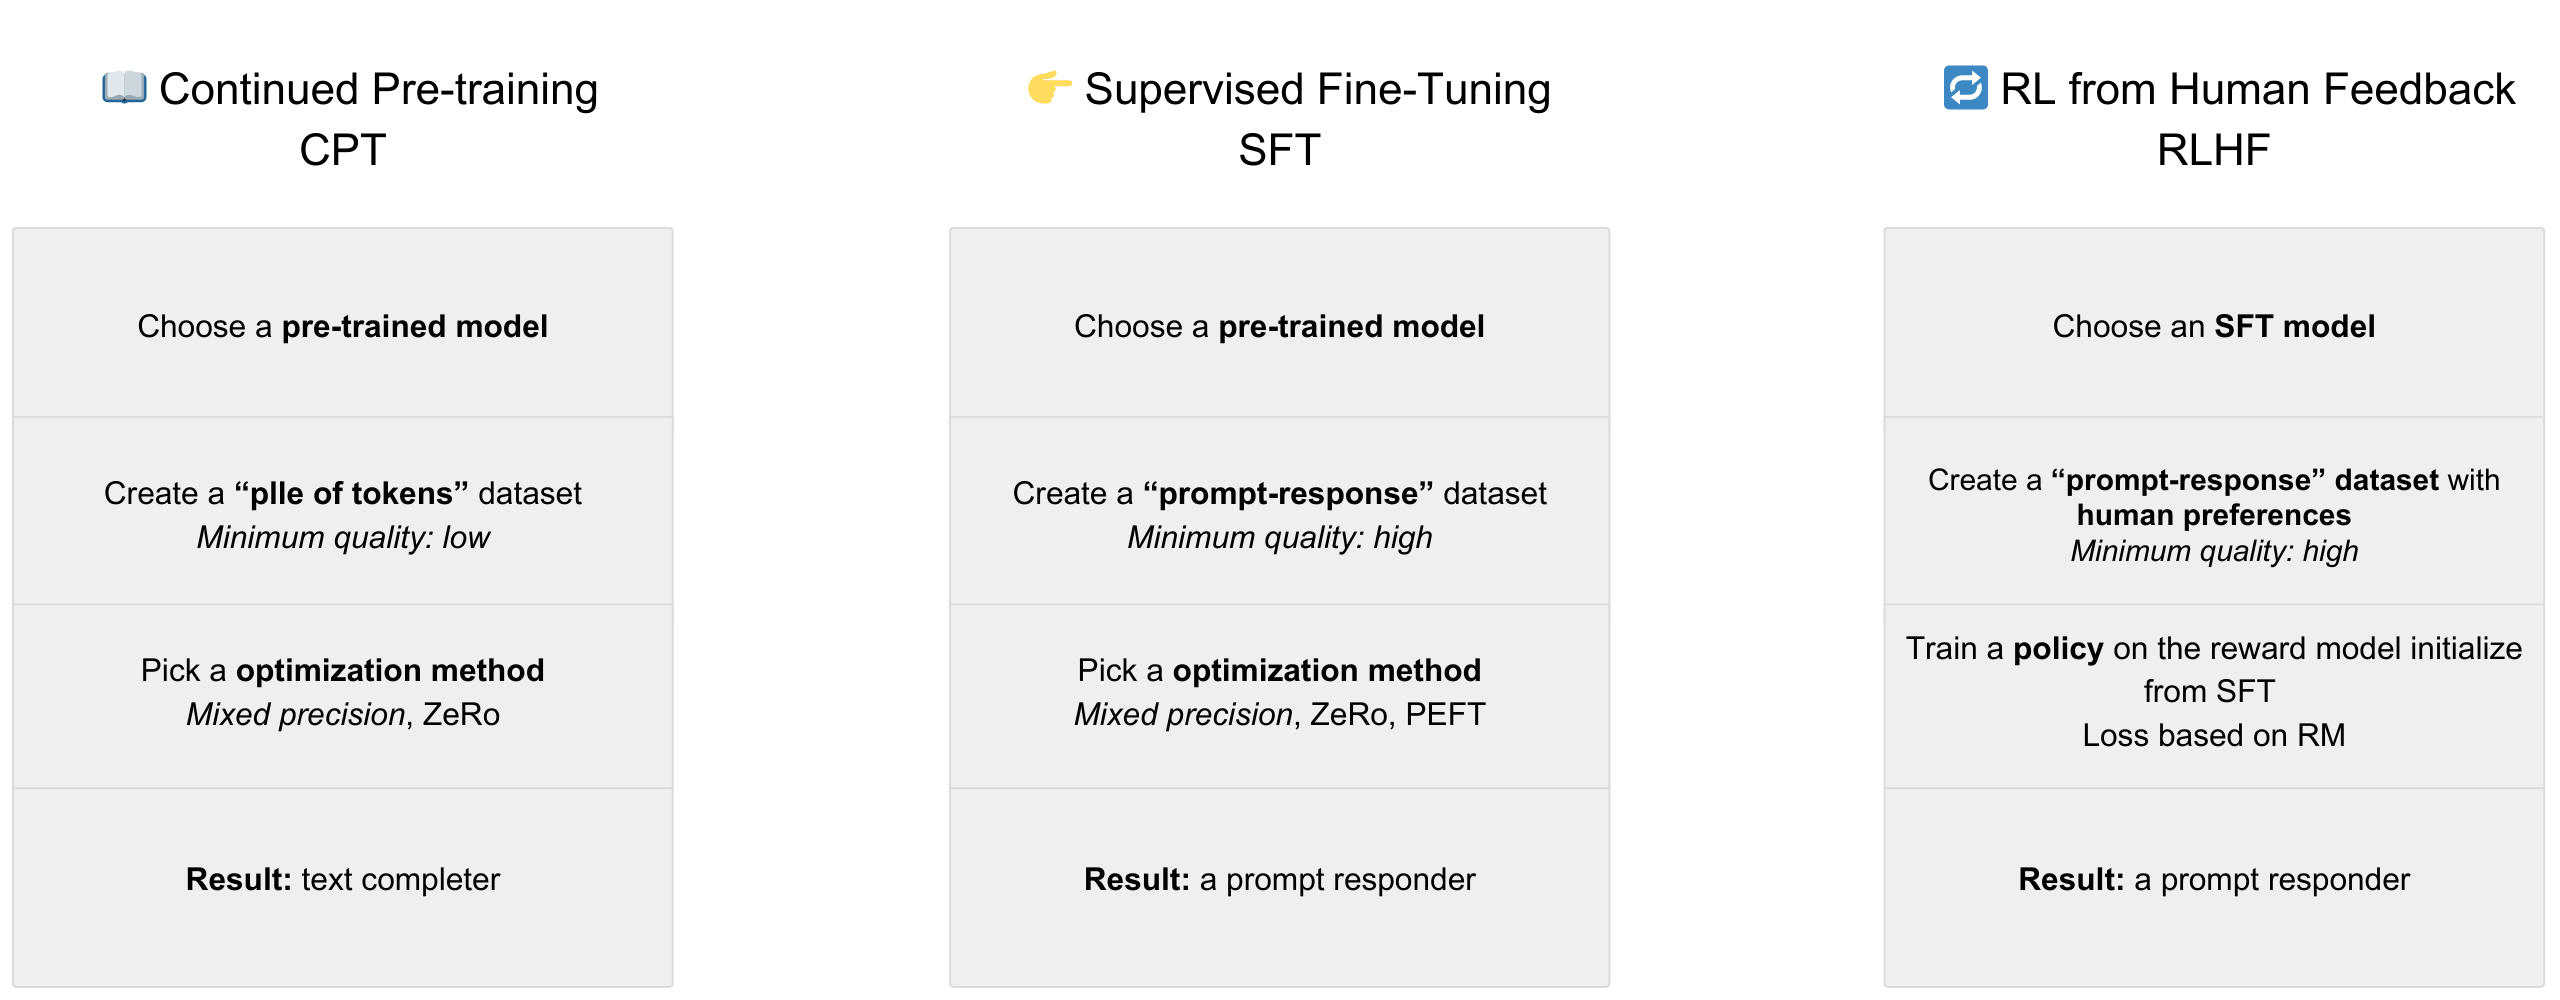
\includegraphics[width=0.8\columnwidth]{logos/comparison.png}
\end{itemize}
\end{block}

    \begin{block}{Fine-Tuning LLM Techniques}
    \heading{Zero Redundancy Optimizer (ZeRO)}
        \begin{minipage}[t]{\textwidth}
            ZeRO involves partitioning the model's parameters across multiple devices or GPUs, enabling parallel processing and reducing memory usage during fine-tuning.
            The model's parameters are divided into separate entities, like optimizer states, gradients, and model weights, which are distributed across different devices.
            This is done in a layer-wise fashion, such that only the model state required for a specific local forward/backward pass is replicated across GPUs. Finally, this process is applied to the backward passes, resulting in updates to the parameters of the model. 
            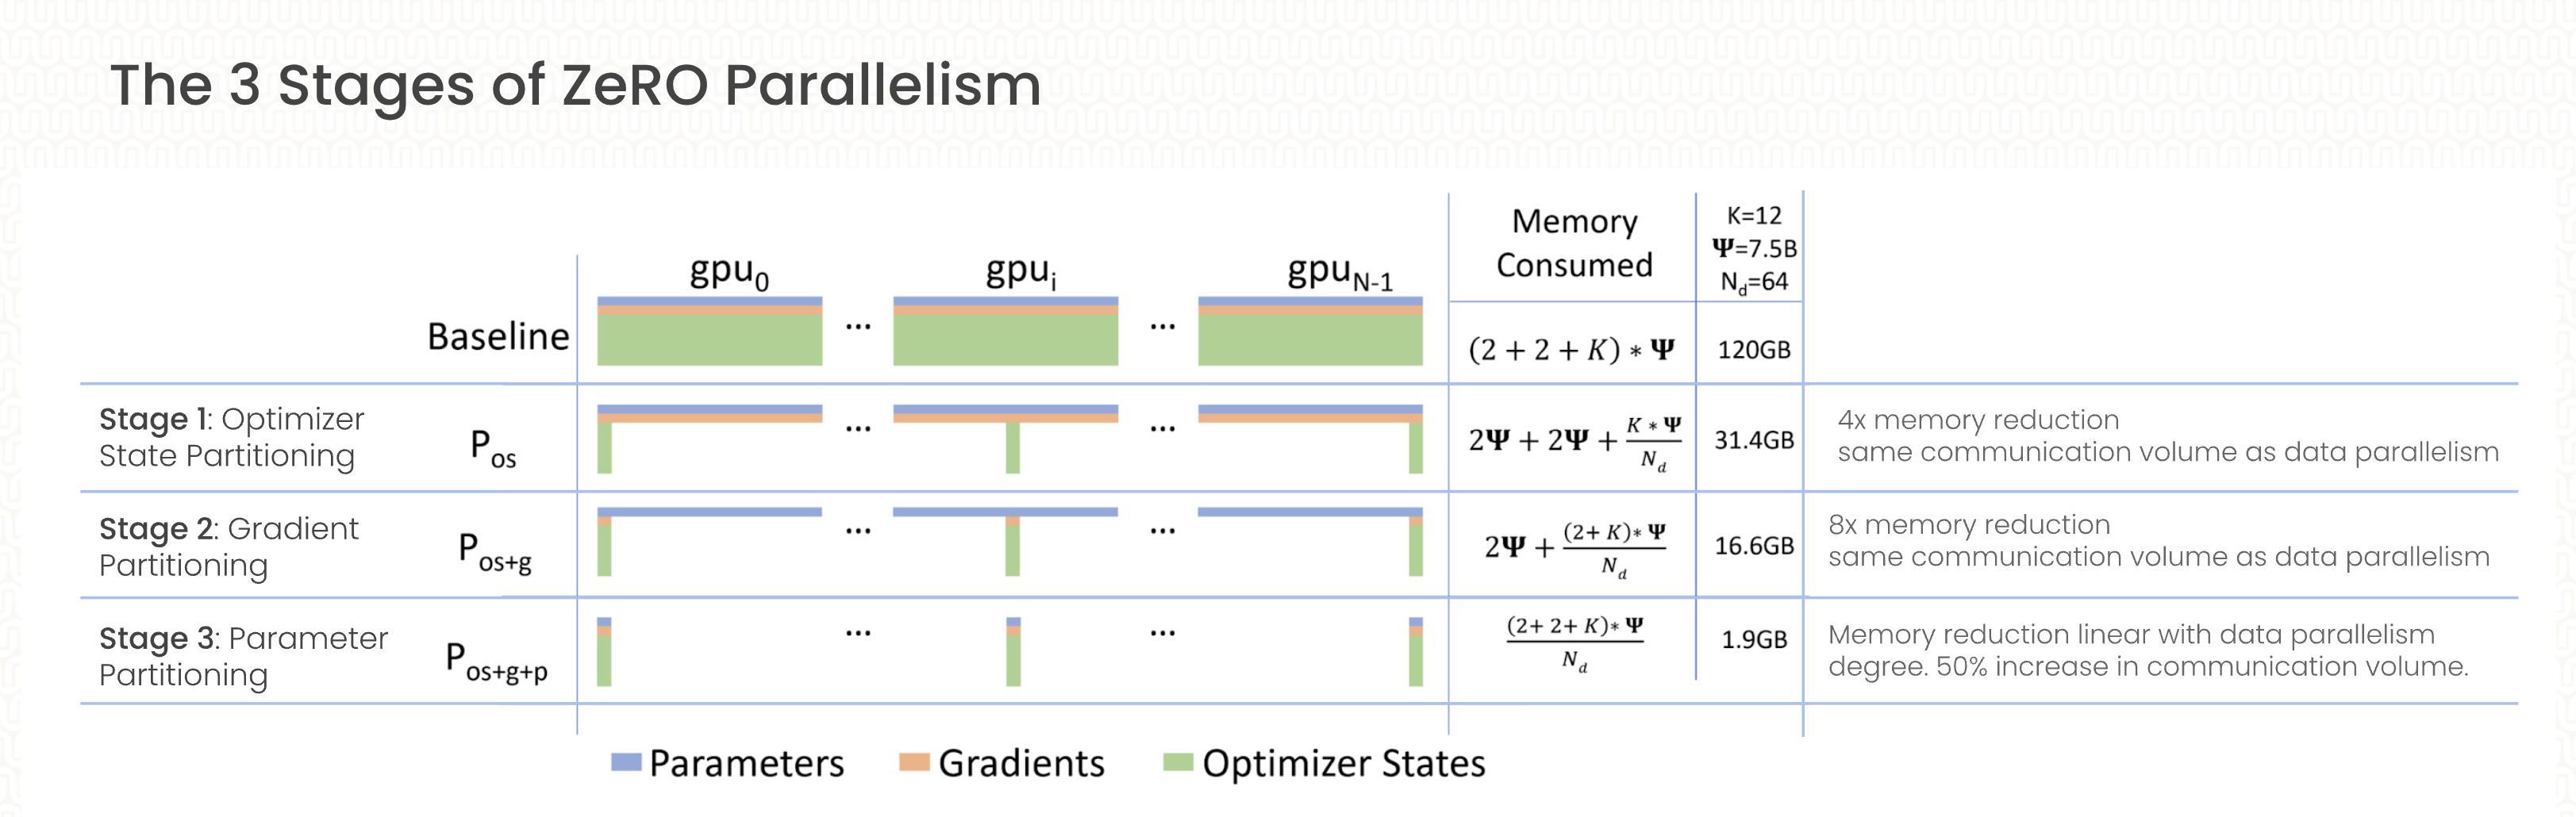
\includegraphics[width=\textwidth]{logos/zero.png}
        \raggedright
        \end{minipage}

        % \begin{minipage}[t]{.30\textwidth}
        % \vspace{-1em}
        %    \begin{figure}[t]
        %    \centering
        %    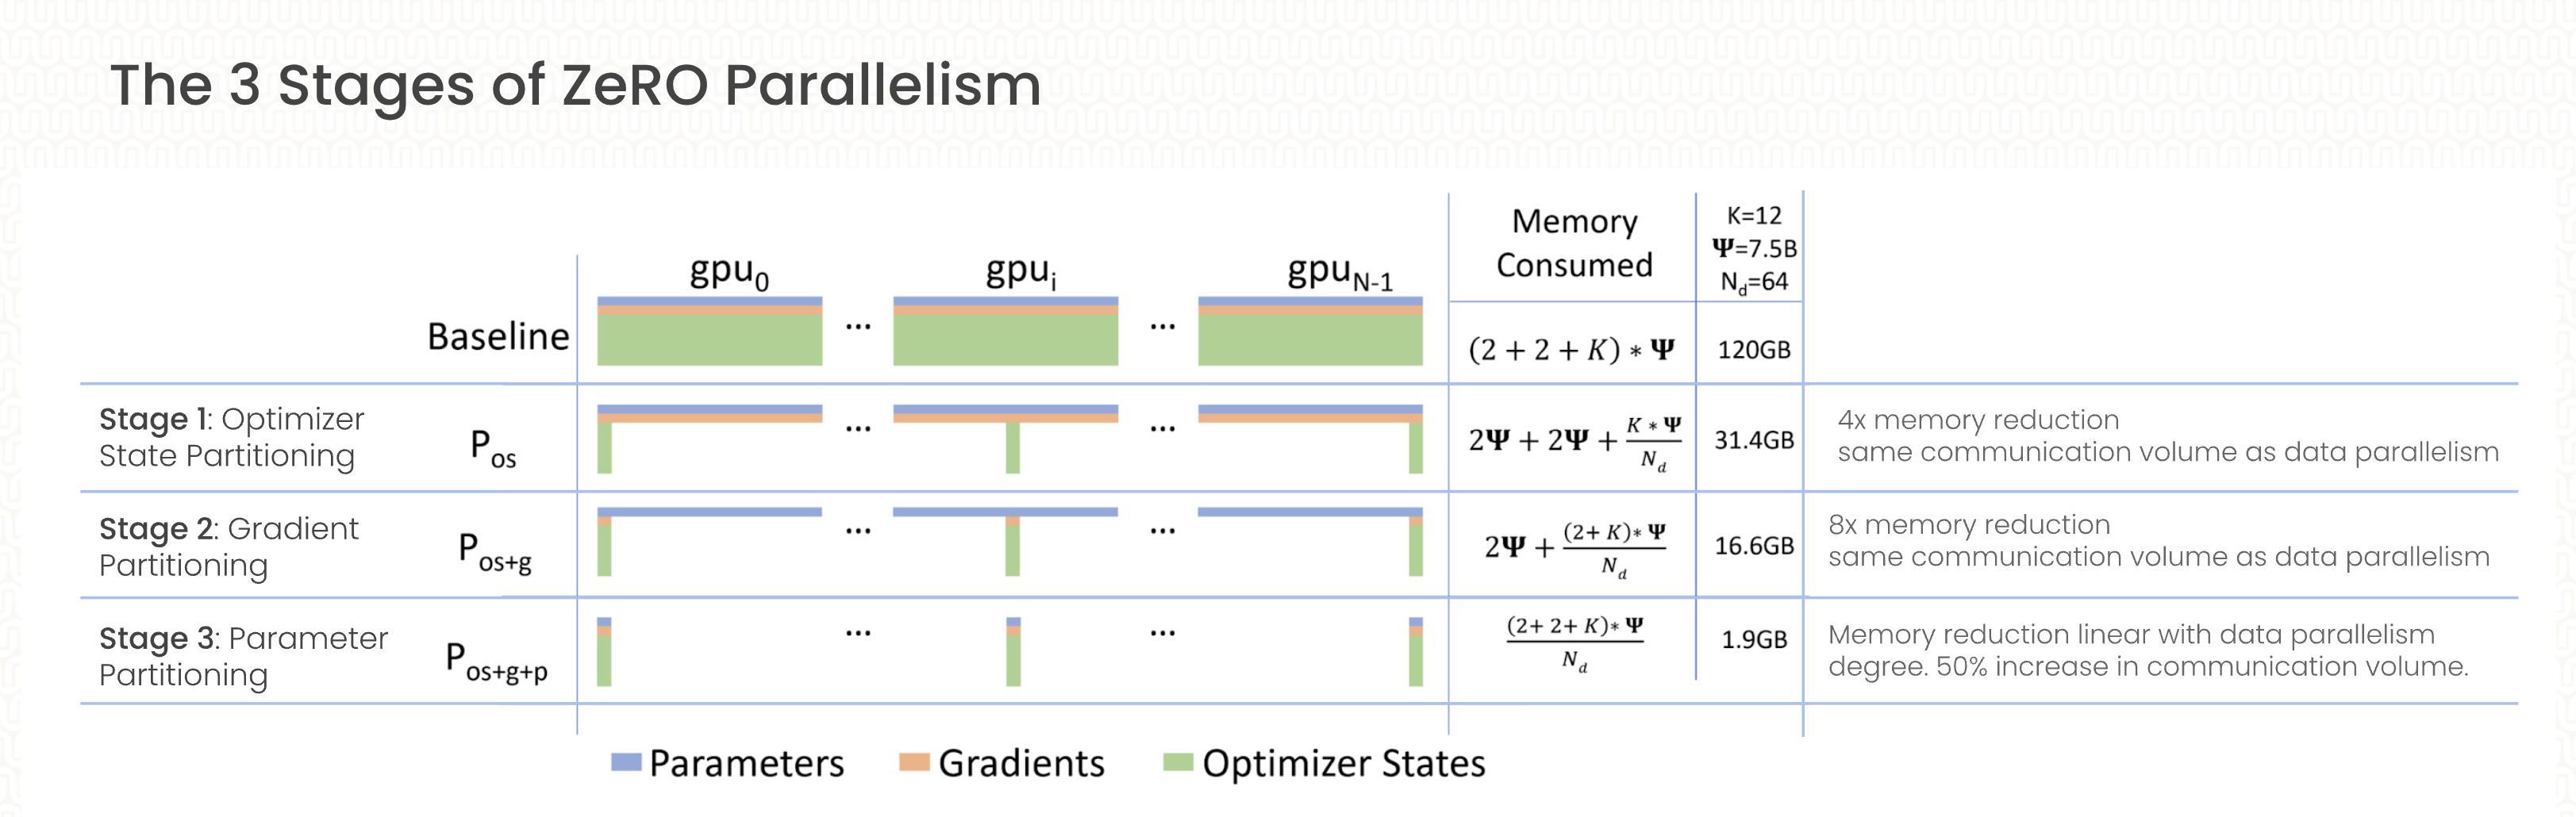
\includegraphics[width=\textwidth]{logos/zero.png}
        %    \end{figure}
        %    \raggedright
        % \end{minipage}\hspace{0.70\textwidth}
    \end{block}
\end{column}

\separatorcolumn

\begin{column}{\colwidth}
    \begin{block}{Fine-Tuning LLM Techniques}
    \heading{8 Bit Quantization}
        \begin{minipage}[t]{.65\textwidth}
            \raggedright
                It involves reducing the precision of the model's parameters from 16-bit or 32-bit floating-point numbers to 8-bit integers, which can significantly reduce the memory required for storing the model's weights. 
                During fine-tuning, 8-bit quantization is applied to the pre-trained model, and only a small number of trainable layers, such as Low-Rank Adapters (LoRA), are added to the model. The gradients are backpropagated through the frozen 8-bit quantized model into the trainable layers, allowing the model to be fine-tuned without modifying the original pre-trained weights
        \end{minipage}
        \begin{minipage}[t]{.30\textwidth}
        \vspace{-1em}
            \begin{figure}[t]
            \centering
            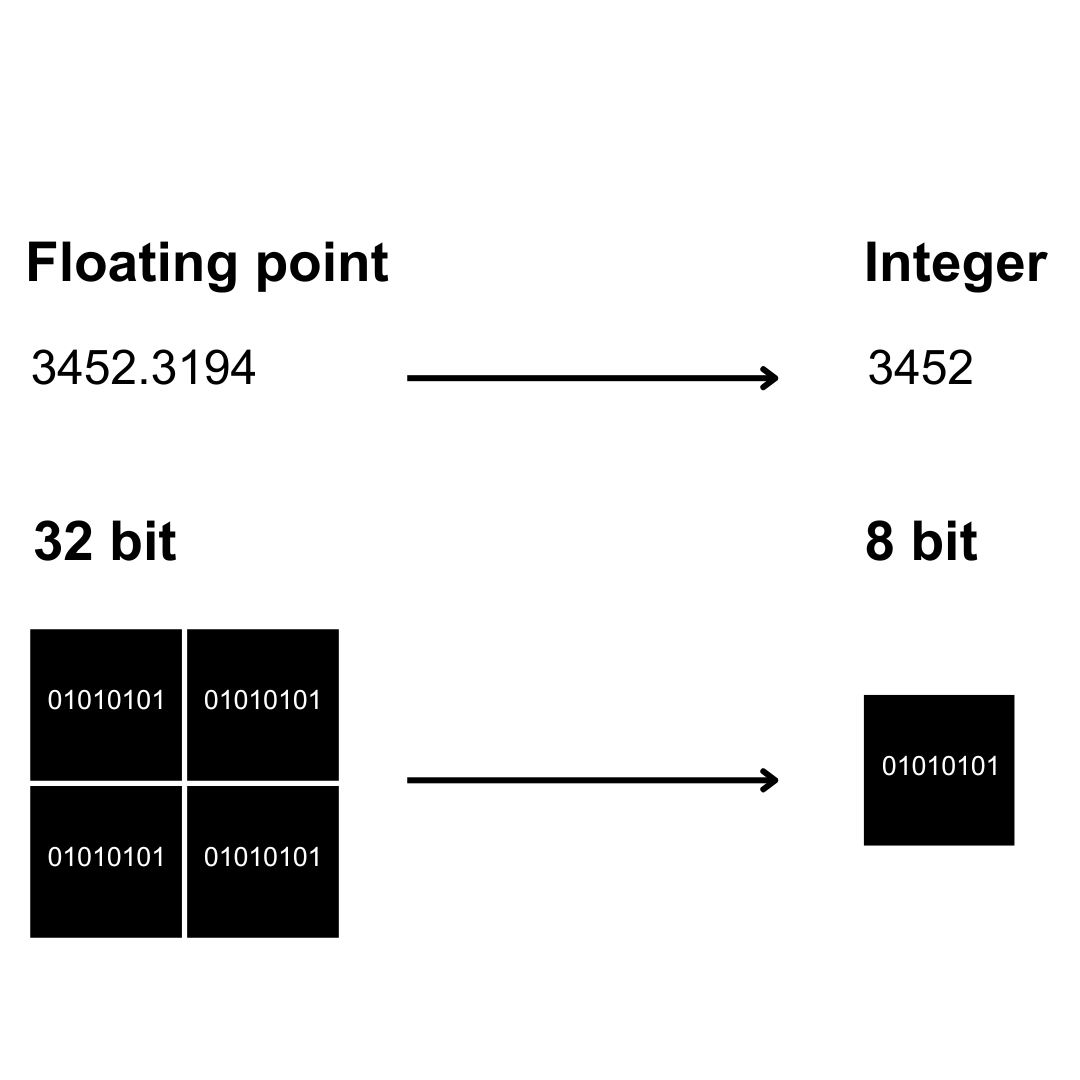
\includegraphics[width=\textwidth]{logos/8bit.png}
            \end{figure}
            \raggedleft
        \end{minipage}\hspace{0.70\textwidth}
        \heading{Parameter-Efficient Finetuning}
        \begin{minipage}[t]{.30\textwidth}
        \vspace{-1em}
            \begin{figure}[t]
            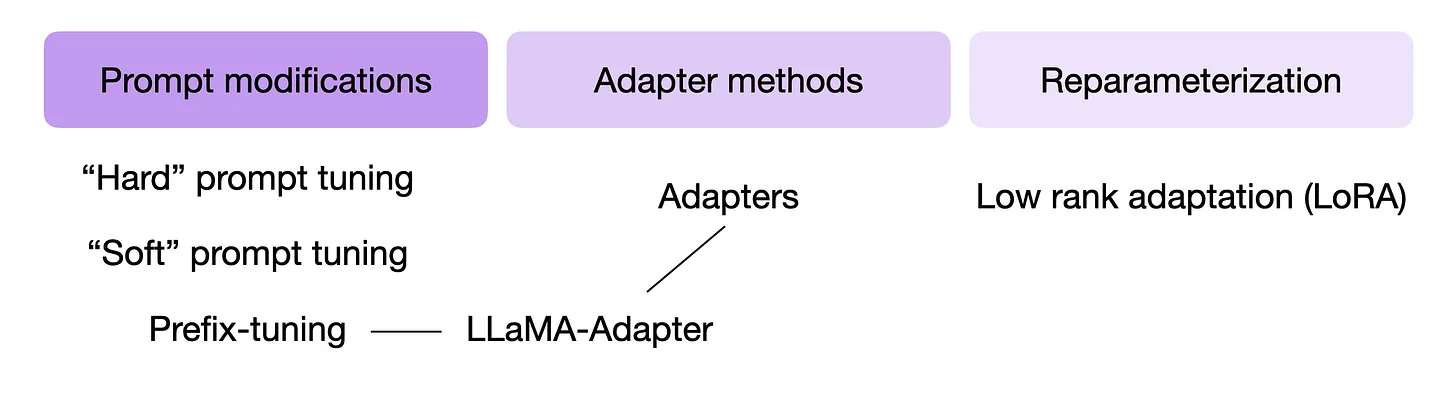
\includegraphics[width=\textwidth]{logos/peft.png}
            \centering
            \end{figure}
            \raggedleft
        \end{minipage}  
        \begin{minipage}[t]{.65\textwidth}
            \raggedright
            Parameter-Efficient Fine-Tuning (PEFT) is a set of techniques used to fine-tune large language models (LLMs) efficiently by modifying only a small subset of the model's parameters. This approach allows adapting pre-trained LLMs to specific tasks without retraining the entire model, which can be computationally expensive and memory-intensive. 
        \end{minipage}
        \heading{Low-rank adaptation (LoRA)}
        \begin{minipage}[t]{.65\textwidth}
            \raggedright
        LoRA operates on the idea that while the weight matrices of LLMs are usually full-rank, the changes made while adapting a model for a specific task usually have lower rank. We learn trainable decomposition matrices that are added to the attention layers of the transformer. This substantially reduces the number of parameters we needed to train in comparison to full fine-tuning, which retrains all parameters. 
        \end{minipage}\hfill
        \begin{minipage}[t]{.30\textwidth}
        \vspace{-1em}
            \begin{figure}[t]
            \centering
            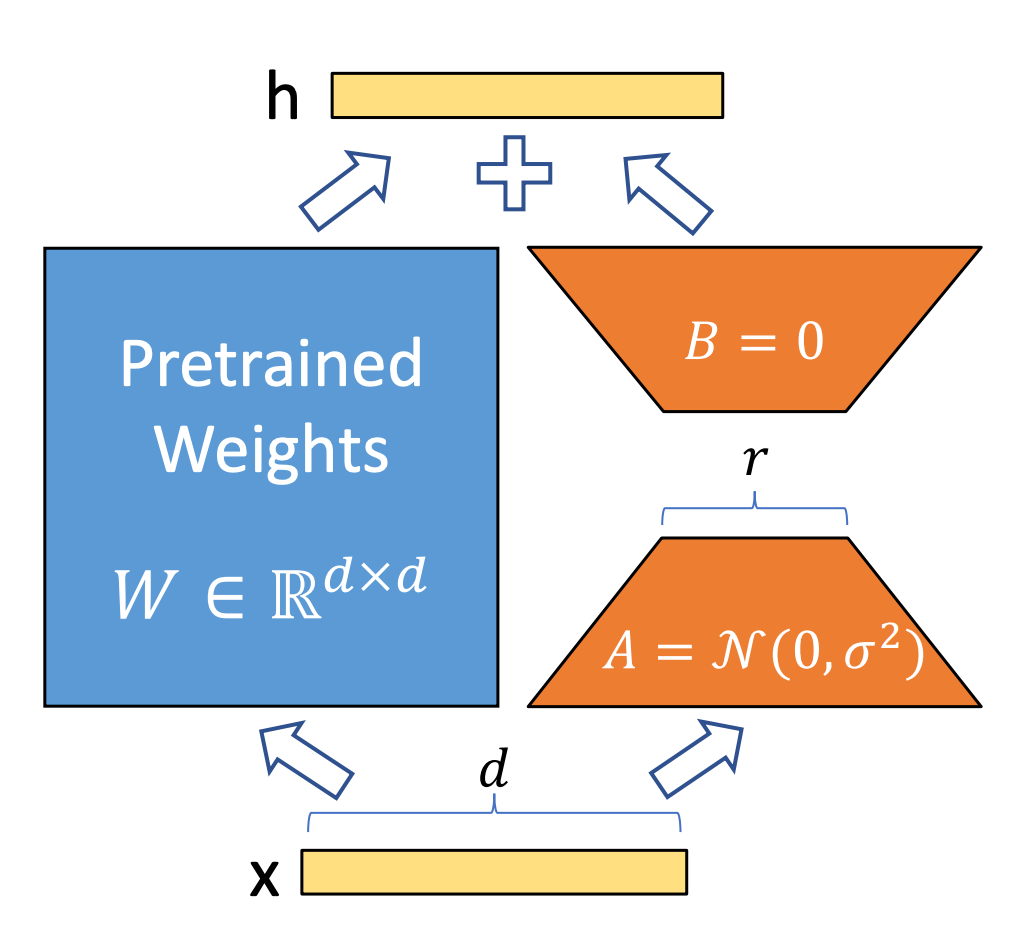
\includegraphics[width=\textwidth]{logos/lora.png}
            \end{figure}
            \raggedleft
        \end{minipage}
        \heading{Q-LoRA}
        \begin{minipage}[t]{.30\textwidth}
        \vspace{-1em}
            \begin{figure}[t]
            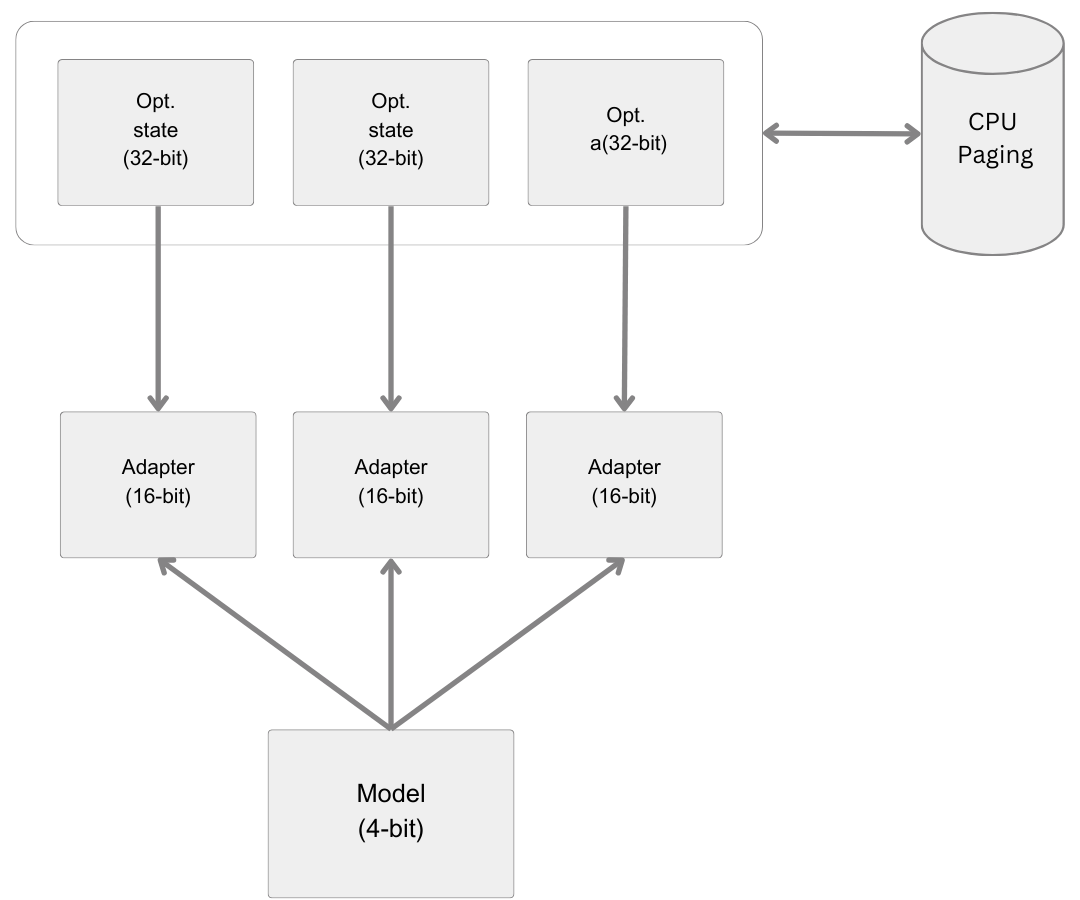
\includegraphics[width=\textwidth]{logos/qlora.png}
            \centering
            \end{figure}
            \raggedleft
        \end{minipage}  
        \begin{minipage}[t]{.65\textwidth}
            \raggedright
            The original model's parameters are quantized to reduce memory usage and computational complexity, while LoRA introduces low-rank tensors with a small number of trainable parameters on top of the frozen original parameters. During fine-tuning, only the parameters in these added tensors are trained, enhancing the model's performance on specific tasks without retraining the entire model. This allows for the quantization of parameters down to 4-bit precision, making it possible to replace the 16-bit base model with a more memory-efficient version
        \end{minipage}
    \end{block}

    
  \begin{block}{The Role of Declarative ML Orchestration}

        ML orchestration isn’t just about DAGs (directed acyclic graphs); it’s also about ensuring that the right computation is done on valid data at the correct time using the appropriate underlying infrastructure. Declarative ML orchestration, in particular, helps you reason about:
        
    \begin{itemize}
    \item The units of computation involved in your overall computation graph
    \item How data is flowing between those units
    \item What exactly those data comprise at any given time
    \item The dependencies each unit applies to its computation
    \item The resources available to each unit 
    \end{itemize}
    
    And it helps you to reason about these things while abstracting away the implementation details of where, when and on what infrastructure the nodes on the graph execute. Orchestrating ML workflows when fine-tuning LLMs ensures each unit of compute is reproducible, repeatable and resource-efficient. An orchestrator like Flyte provides a flexible and powerful platform that unifies data, ML and analytics stacks.

    Check out about Flyte here: https://github.com/unionai-oss/llm-fine-tuning

    How Pieces implements LoRA: https://code.pieces.app/blog/lora-ai-and-generated-labels
  \end{block}

\end{column}

\separatorcolumn

\begin{column}{\colwidth}

  \begin{exampleblock}{Using Flyte to do LLM Finetuning}
Flyte is a production-grade orchestrator that unifies data, ML, and analytics stacks. It supports tools like pandas, pytorch, pyspark and plotly so that you can integrate them all into your workflows.

Flyte facilitates efficient LLM fine-tuning through declarative resource allocation (GPUs, CPUs), containerized environments (ImageSpec), caching, and cost-saving features (spot instances, checkpointing). Integration with LLM libraries (hugging face) and monitoring tools (Flyte decks) simplifies model management and analysis.

\begin{figure}
\centering
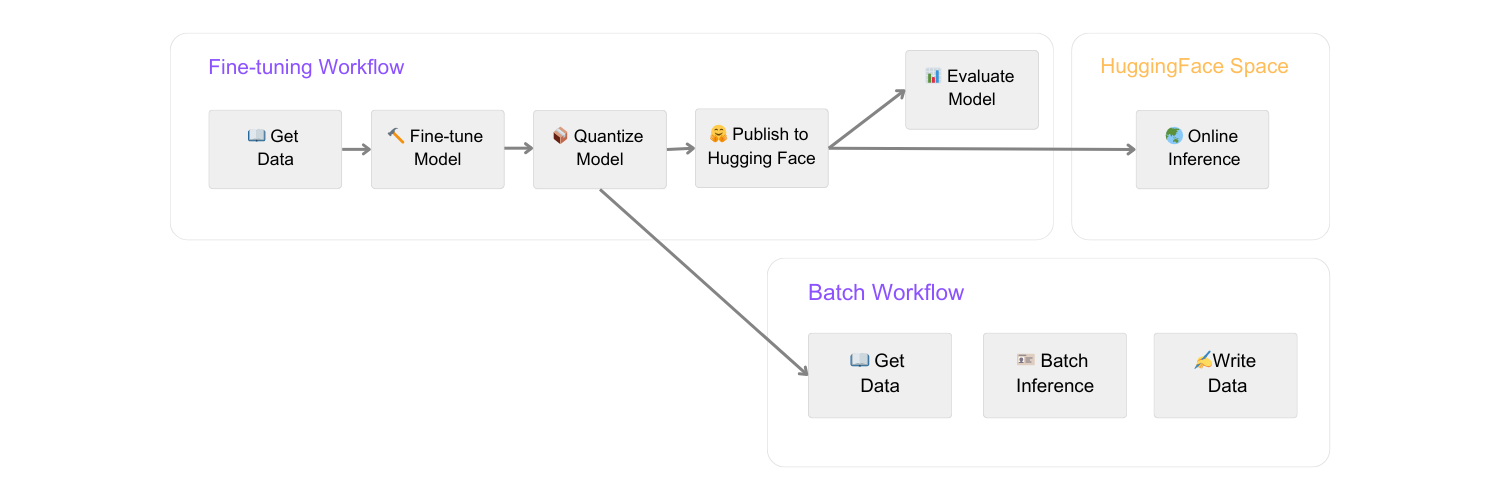
\includegraphics[width=0.7\columnwidth]{logos/flowchart.png}
\end{figure}
\end{exampleblock}

  \begin{block}{Code}

    \begin{document}
\begin{minted}[fontsize=\small]{python3}
import transformers
from dataset import Dataset
from transformers import Trainer, TrainingArguments
from flytekit import task, workflow

def train(
    config: TrainerConfig, dataset: Dataset, 
    deepspeed_config: Optional[dict] = None
    ) -> flytekit.directory.FlyteDirectory:  
  train_dataset, eval_dataset = split_data(dataset)
  model = transformers.AutoModelForCausalLM.from_pretrained(config.base_model)  
  tokenizer = transformers.AutoTokenizer.from_pretrained(config.base_model, **tokenizer_kwargs)
  training_args = TrainingArguments ( learning_rate=config.learning_rate, fp16=config.fp16, ...)
  trainer = Trainer(
      model=model, tokenizer=tokenizer, args=training_args, train_dataset=train_dataset,
      eval_dataset=eval_dataset,)
  trainer.train()
  trainer.save_model(output_dir=config.output_dir)
  return flytekit.directory.FlyteDirectory(path=output_dir)

def get_data(config: TrainerConfig) -> Annotated[StructuredDataset, PARQUET]:
  dataset = load_dataset(config.data_path, config.data_name,)
  pd_dataset = dataset["train"].to_pandas()
  try:
    WikipediaDataset.validate(pd_dataset, lazy=True)
  except pa.errors.SchemaErrors as exc:
    flytekit.Deck("pandera-errors", TopFrameRenderer(max_rows=100).to_html(exc.failure_cases))
  flytekit.Deck("dataset", HuggingFaceDatasetRenderer().to_html(dataset["train"]))
  return StructuredDataset(dataframe=dataset["train"])

def fine_tune(config: TrainerConfig,
    deepspeed_config: Optional[dict] = None,) -> str:
    data = get_data(config.config)
    model_dir = train(config=config, dataset=data, deepspeed_config=deepspeed_config,)
    quantized_model_dir = quantize_model(config.config, model_dir=model_dir)
    save_to_hf_hub(model_dir=model_dir, config=config)
    save_to_hf_hub(model_dir=quantized_model_dir, config=config, quantized_8bit=True)
    return model_dir
    
@task(requests=Resources(mem="8Gi", cpu="2", ephemeral_storage="8Gi"),
    disable_deck=False, cache=True, cache_version="0.0.0",)
    
def get_data(config: TrainerConfig) -> Annotated[StructuredDataset, PARQUET]:
    ...
@task(retries=3, cache=True, cache_version="0.0.0", 
requests=Resources(mem="256Gi", cpu="64", gpu="8", ephemeral_storage="200Gi"),
    task_config=Elastic(
        nnodes=5, nproc_per_node=8,
        rdzv_configs={"timeout": 3600, "join_timeout": 3600},
        max_restarts=1,),)
        
def train(config: TrainerConfig, dataset: Dataset, deepspeed_config: Optional[dict] = None) ->
flytekit.directory.FlyteDirectory:
    ...
@workflow
def fine_tune(config: TrainerConfig, deepspeed_config: Optional[dict] = None):
    ...
\end{minted}
\end{document}

  \end{block}

\end{column}

\separatorcolumn
\end{columns}
\end{frame}
\end{document}